%!TEX root = ../dissertation.tex
\Chapter{Conclusion}
\label{conclusion}




\section{Other approaches to optimal sequential models of cognition}



\subsection{POMDP}\label{sec:alternative-pomdp}


\section{Points of weakness and avenues for growth}

There are several dimensions on which the framework could be extended in future work.

\subsection{Learning the metalevel homunculus}

One of the most significant challenges for the metalevel MDP framework is the problem of infinite regress. As mentioned in the Introduction (Section~\ref{sec:bound-meta}), the framework assumes that people are \emph{metalevel rational}, meaning that they choose computational actions to optimally balance a cost-benefit tradeoff. However, it does not explain how those choices are themselves made. In this way, the framework assumes a ``metalevel homonculus'': an unbounded, perfectly rational agent that always knows just what thought to think next (c.f. \citealp{hazy2006banishing,botvinick2014computational}). Explaining (or perhaps explaining away) the homonculus is critical for these models to provide a complete explanation of how people effectively allocate computational resources.

Perhaps the most plausible theory of the metalevel homonculus is that it is learned. Indeed, learning has been a critical aspect of many models of metalevel control in psychology. The earliest examples are found in cognitive architectures like ACT-R and SOAR, which have simple mechanisms for learning when to apply different production rules \citep{laird1986chunking}. However, like early models of strategy selection \citep{shrager1998scads}, this type of learning was primiarily associative. The idea that a metalevel controller explicitly learns to maximize reward was proposed in later strategy selection models \citet{erev2005adaptation,rieskamp2006ssl,lieder2017strategy}. Reinforcement learning (RL) has also been proposed as the mechanism by which the brain learns which goals to pursue \citep{cushman2015habitual}, and when to retrieve and store information in working memory \citep{oreilly2006making,todd2008learning} and episodic memory \citep{lu2022neural}. 

Metalevel MDPs provide a natural framework in which to cast theories of metacognitive RL. However, expliciting formalizing the metalevel control problem in this way also reveals a major challenge: learning good policies in metalevel MDPs is very challenging. They tend to have very large (mental) state spaces, and they have highly stochastic dynamics. Perhaps most challenging, however, is the temporal credit assignment problem. In each episode, the agent takes many computations, but receives only a single external reward. It is thus not clear which computations should receive ``credit'' for large rewards. 

One way to make learning easier in the presence of sparse rewards is to adjust the reward function, adding \emph{shaping rewards} (or ``pseudo rewards'') that provide more immediate feedback about the value of each (mental) action that is executed \citep{ng1999policy}. We have shown that shaping rewards derived from the optimal metalevel value functions can accelerate human learning in the Mouselab MDP task used in Chapter~\ref{sec:planning} \citep{callaway2022leveraging}. Although people would not have access to such perfect shaping rewards in the real world, they may have access to simpler but still useful surrogates.\footnote{%
  \citet{hay2016principles} propose one intuitively appealing shaping reward based on the difference in the expected value of taking an external action in the mental states before and after executing a computation. However, the results were, in his terms, ``not yet as good as we’d like''.
} That is, people may experience a reward when they have a ``good thought'' even if it does not immediately lead to an external action \citep{gopnik1998explanation}. Indeed, people appear to place value on external information that cannot be acted on \citep{eliaz2007experimental,gottlieb2018neuroscience}, and we have begun to formalize the specific qualities of information that people value \citep{markant2014preference,markant2016selfdirected}. This suggests a fascinating research question: what factors elicit the subjective experience of having a good thought?


\subsection{Partially observable minds}

% A key assumption of the metalevel DMP framework is that the agent has direct access to the mental state. Indeed, 

A key structural assumption in the framework is the distinction between the mental state and the world state. The defining features of the mental state are that it can be affected by computation, and that it is directly accessible to the agent. However, these two features do not need to come together. It is possible that we do not have complete access to aspects of our mental state that we can nevertheless control to some extent. This possibility was suggested by \citet{suchow2016deciding}, who proposed a POMDP model of working memory maintenance. In this model, the agent selects mental actions to increase the activation level of a selected memory, but the current activation levels can only be imperfectly measured. This model did not invoke a notion of world states or external actions, however.

To allow for partial observability in a metalevel MDP, we can simply assume that the agent does not have direct access to the mental state, but instead has access to an incomplete observation of that state. An interesting question arises as to how these observations should be used. From a POMDP perspective, the observations should be integrated over time into a metalevel belief state (a distribution over mental states). However, this complicates the metalevel controller considerably, creating technical challenges in finding optimal solutions, and exacerbating the homonculus problem described above. An alternative approach, employed by \citet{suchow2016deciding}, is to assume that the metalevel decisions are made based only on the current observation. This yields a simpler and perhaps more psychologically plausible model. However, because observations are not Markovian, one could no longer use standard dynamic programming techniques to find the optimal policy. This further motivates the development of model-free strategies for learning metalevel policies.

\begin{figure*}
  \centering
  \includegraphics[width=0.8\textwidth,page=2,trim=0 100 0 50]{diagrams/metamdp.pdf}
  % 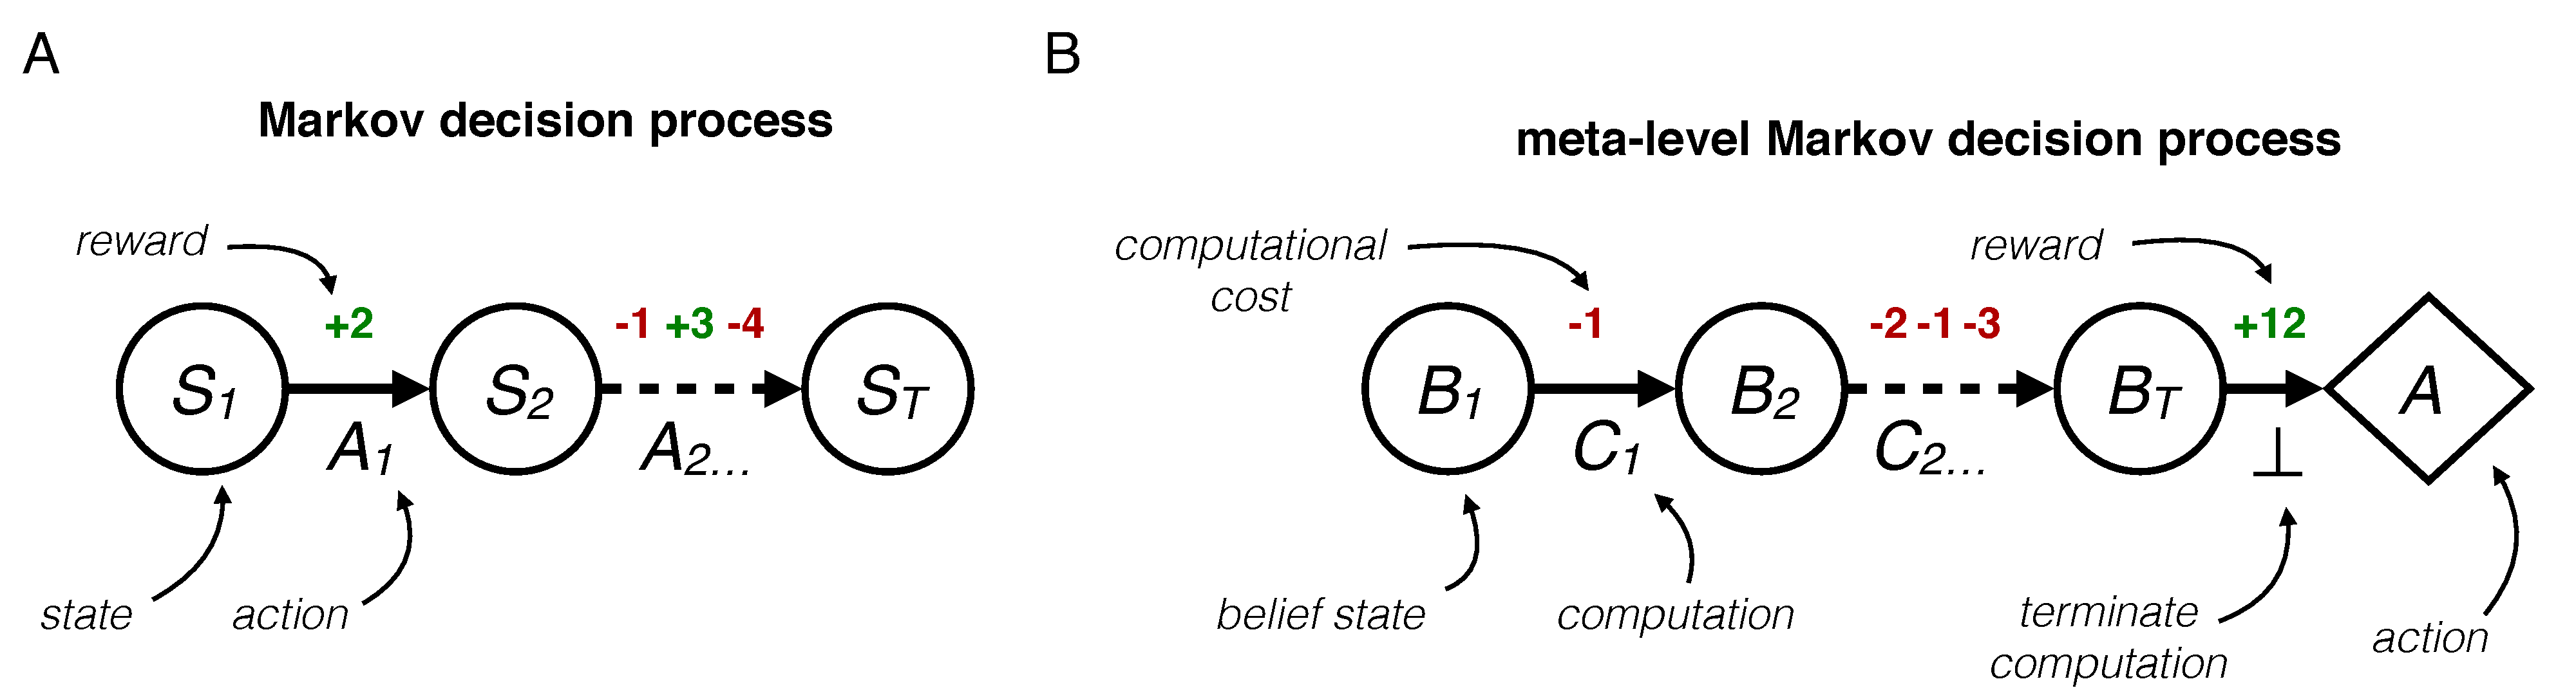
\includegraphics[width=\textwidth]{figs/metamdp.pdf}
  \caption{\captiontitle{Interleaved metalevel MDP}. To formalize the problem of interleaved computation and action, we can augment the metalevel MDP framework to include sequences of world states, actions, and external rewards. Note that there is no cognitive cost in this formalism, as any opportunity costs should be captured in the external reward function. The elements that capture the external environment are indicated in blue.
  }
  \label{fig:metamdp-joint}
\end{figure*}

\subsection{Interleaved computation and action}

A second key structural assumption in the framework is that each metalevel episode occurs within a single external timestep. That is, the world state does not change, and only one external action is executed (at the end of the episode). This has two implications. First, it assumes that the agent can think as long as they want without having to worry about the world state changing. Second, it assumes that information considered while choosing one action cannot influence the selection of future actions. Although these assumptions hold approximately in many experimental and naturalistic tasks, they will not hold in fast-paced dynamic problems (e.g. jay walking) or in sequential problems with stochastic dynamics (e.g. chess).

To model interleaved computation and action, we essentially replace the single world state and action with a full external MDP that progresses in lockstep with the metalevel MDP (c.f. joint-state MDPs; \citealp{russell1991right,parr1998reinforcement,hay2016principles}). Figure~\ref{fig:metamdp-joint} illustrates one way this could work. At each timestep the agent selects both a computation and an action (the action may be to simply sit still while thinking). The next world state and reward depend on the current state and action, as in a standard MDP. As before, the next mental state depends on the current mental state and the computation executed; it additionally depends on the previous action and the \emph{new} world state. The former captures the fact that the agent may understand how their actions affect the world. The latter captures the agent's ability to perceive the changing world state.

In the interleaved case, the decision about how much to think becomes more nuanced. Specifically, one must not only decide \emph{how much} to think but also \emph{when} to think. In some cases, it may make sense to do all of one's thinking up front, as the standard metalevel MDP assumes. This strategy makes sense because it ensures that every action you take is informed by all the computation you do. However, there are at least three reasons one might want to begin acting before having a complete plan. First, one may be able to continue thinking while executing the early part of the plan, for example considering which way one will turn while walking down a long corridor \citep{oceallaigh2015metareasoning}. Second, if the world dynamics are stochastic, knowing how those transitions unfold will allow the agent to focus their planning on the the situtation the agent actually encounters. Third, forming a complete plan may impose representational costs that could be avoided by only constructing a concrete plan for the immediate future, perhaps having a more abstract plan for the more distant future \citep{ho2020efficiency}.

\subsection{Optimizing the architecture}

A third assumption of the framework is that only the policy, and not the metalevel MDP itself, is optimized. This assumption is almost always made in standard applications of MDPs, as the MDP represents the external environment, which the agent has no direct control over. In contrast, beccause a metalevel MDP represents an agent's internal computational environment, it is likely that the metalevel MDP itself is adapted to the structure of the external problems the agent has to solve.

There are two timescales at which adaptation of an organism's cognitive architecture could occur (in animals): evolutionary and developmental. Clearly, evolution has a major role in shaping the total amount of biological resources allocated to cognition (e.g., brain volume), as well as the ease with which certain types of computations can be learned and executed. However, at the level of abstraction that we have posed metalevel MDPs, the developmental timescale is likely to be more relevant. Indeed, it is natural to view many types of learning as a process of developing new mental states and computational actions. For example, as a consequence of reading this dissertation, you have (hopefully) acquired a computation along the lines of ``identify the computational actions in this cognitive model''.


\section{Final remarks}



